\documentclass[border=12pt]{standalone}
\usepackage{amsmath,amssymb,tikz-feynman}
\tikzfeynmanset{compat=1.1.0}
\begin{document}
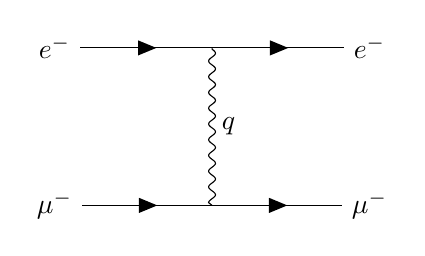
\begin{tikzpicture}
\begin{feynman}
\vertex (i1) at (-2,1) {$e^-$}; \vertex (o1) at (2,1) {$e^-$};
\vertex (i2) at (-2,-1) {$\mu^-$}; \vertex (o2) at (2,-1) {$\mu^-$};
\vertex (a) at (0,1); \vertex (b) at (0,-1);
\diagram*{ (i1)--[fermion](a)--[fermion](o1), (i2)--[fermion](b)--[fermion](o2), (a)--[photon,edge label={$q$}](b) };
\end{feynman}
\end{tikzpicture}
\end{document}
